\documentclass[a4paper,12pt]{report}
\usepackage[T1]{fontenc}
\usepackage[utf8]{inputenc}
\usepackage{pslatex}
\usepackage{lmodern}
\usepackage{helvet}
\usepackage{geometry}
\usepackage{graphicx}
\usepackage{sectsty}
\usepackage{fancyhdr}
\usepackage{titlesec}
\usepackage{fixltx2e}
\usepackage{acronym}
\usepackage[titles]{tocloft}
\usepackage{amsmath}
\usepackage{amssymb}

\usepackage{cases}
\usepackage{cite}
\usepackage[export]{adjustbox}
\usepackage{url}
\usepackage{rotating} 

\usepackage{setspace}
\usepackage{booktabs}

\usepackage{float}
\usepackage[ruled,vlined,linesnumbered]{algorithm2e}

\chapterfont{\large\centering}
\sectionfont{\normalsize}
\subsectionfont{\normalsize}
\linespread{1.5}
\geometry{a4paper,left=3cm,right=2cm,top=2cm,bottom=2cm}
\setcounter{tocdepth}{2}
\usepackage{amsmath}
\begin{document}
\pagenumbering{roman}
\setcounter{page}{1}
\setcounter{tocdepth}{1}
\renewcommand\contentsname{CONTENTS}
\tableofcontents

% EDIT THIS
\newpage
\vspace*{2.52cm} \hspace*{-0.88cm}
\addcontentsline{toc}{chapter}{LIST OF ABBREVIATIONS}
\hspace*{4.3cm}
\textbf{{\large LIST OF ABBREVIATIONS}}\\
\vspace*{0.5cm}
\begin{acronym}[AWGN]
	 \acro{ANN}{Artificial Neural Network}
     \acro{CNN}{Convolutional Neural Network}
     \acro{OCR}{Optical Character Recogntion}
     \acro{GNU}{GNU Not Unix}
     \acro{KDE}{K Desktop Environment}
     \acro{GNOME}{GNU Network Object Model Environment}
     
\end{acronym}

\newpage
\addcontentsline{toc}{chapter}{LIST OF FIGURES}
\renewcommand\listfigurename{LIST OF FIGURES}
\listoffigures

%INTRODUCTION
\newpage
\pagenumbering{arabic}
\setcounter{page}{1}
\renewcommand\chaptername{CHAPTER}
\chapter{INTRODUCTION}
A bus  is a road vehicle designed to carry a large number of passengers. The services offered by the buses has made it the most preferred mode of transportation for the citizens. The cheap ticket fares, the convenience, the safety and a capacity as high as 300 passengers  has made buses a desirable choice for travel by the citizens. The reason behind their wide usage is, the cheap ticket fares, the
convenience as well as the safety being ensured for passengers. Being a local service, the buses display the destinations in their native language. Unfortunately, foreigners along with people who are unable to comprehend the native language find it difficult to use the local bus service.

\paragraph{}
The project focuses on developing a software solution that will help end users to navigate across a city by integrating with the local bus service. Our aim is to help the target users overcome this difficulty. We aspire to improve the bus service not only for the citizens but also for our target users and to help their travel easier.

\section{Problem Statement}
Around 30\% of the population comprises of foreigners and people who are unable to comprehend the native language, thereby making it difficult for this group to understand the locations written on the bus boards. Our main aim is to provide a software solution that will: 

\begin{itemize}
\item help end users to navigate across a city by representing the destinations in the English language which is known to all
\item provide bus stop destinations to the end user
\item provide accurate location of the destination
\end{itemize}

\section{Motivation}
Kerala is rated as the most popular tourist destination in India by international travellers who cite beaches, Ayurveda resorts and spas as the prime attractions. Statistics related to the arrival on tourists in Kerala is a good way to measure the growth of the sector over a certain period of time. Foreign tourist arrival to Kerala during 2017 crossed 10.91 lakhs which marked an increase of 5.15\% over the previous year. It is observed that there is a consistent growth in foreign tourist arrival in Kerala. Figure 1.2. as given below indicates the arrival of foreign tourists to Kerala during the last five years and percentage of variation over the previous year. 

\vspace*{0.2cm}
\begin{figure}[!h]
	\begin{center}
		\includegraphics[width=12cm , height= 6cm]{graph.png}    
		\caption{Growth of foreign tourists}
		\label{fig1}
	\end{center}
\end{figure}
\vspace*{0.5cm}

Hence the primary motivation for our project targets this group as end users. Foreign tourists as well as residents in Kerala who wish to commute via bus service require basic understanding of the Malayalam language. Also people who are unable to comprehend the language find it difficult to use this service. 

\section{Objectives}
The core objectives of this project are listed below:
\begin{itemize}
\item provide user friendly interface
\item understanding of Malayalam scripts
\item language translation to common English language
\item time and cost efficient
\item increase effectiveness
\item reliability of service
\item ease of use
\end{itemize}

\section{Optical Character Recogntion}
OCR is the automated translation of images of typed, printed or handwritten text into coded text, whether from a scanned document, a photo of a document,  from subtitle  text  overlying  on  an  image. There  are  many  methods  of  OCR  to recognise character like thinning, thickening, pre-processing, feature extraction, 
feature vector, segmentation and so on. 
OCR is a technology that recognizes text within a digital image. This approach is implemented in our project to detect Malayalam characters from the digital images of the bus boards. The images of the bus boards are converted to digital greyscale images. A standard deep learning approach of OCR is used for this purpose. A CNN model is trained with a dataset of Malayalam characters. On providing a test image of a Malayalam character, it detects the desired character. 

\section{Overview}
The report mainly discusses the current state of the project. The Literature Review will discuss about the various Research Papers and the various concepts the team has evaluated to solve the problem. Each of the team member was given different topics to review and the top three relevant paper has been reviewed discussing the valuable contribution from each. The Dataset chapter discusses the Dataset we are considering for this project and the various advantages over similar datasets. The Design chapter will discuss about the various use cases and requirements of the project and how that is solved by our design. The Action Plan discusses about the project management style adopted and how the timeline for the project has been designed. It also discusses in detail about the various principles followed by the project.The report is concluded with all that is discussed and the further work that is to be taken in the Conclusion chapter. And the citations for the research papers are presented in the References chapter.


\renewcommand\chaptername{CHAPTER}
\chapter{LITERATURE REVIEW}

Optical character recognition is one of the litmus tests of pattern recognition algorithms. In addition to pattern recognition, optical character recognition involves some other fields of knowledge, such as image processing, artificial intelligence and linguistics \cite{Jader,Goodfellow,Hu}. Optical character recognition can make computers handle real world texts directly. The research results can be applied to a large number of practical problems, such as mail splitting, check recognition, image retrieval, intelligent robots and handwriting input. Commonly used methods in character recognition can be divided into three categories: template matching; feature extraction and classification; and deep learning methods. In the template matching method, a standard template set is first established for the character to be recognized, and then the preprocessed images of the character to be recognized are sequentially projected onto the templates for matching. The best matching template corresponds to the character being recognized. Feature extraction and recognition are the most commonly used methods in optical character recognition. The process consists of two parts. The first step uses an algorithm to extract the features of the character image. The commonly used feature extraction algorithms are: SIFT, SURF, and HOG. The second step is to use a classifier to classify the acquired features. Common classifiers include the Bayesian classifier, support vector machine, K nearest neighbor algorithm, artificial neural network algorithm, etc. \cite{Nas} Deep learning has become the most commonly used method since its appearance. The most commonly used deep learning model in the field of character recognition is the convolutional neural networks.

\paragraph{}
A CNN is a feedforward neural network inspired by biological processes. Unlike traditional network architectures, a CNN contains very special convolution and down sampling layers \cite{Cire}. LeNet5 was born in 1994 and is one of the earliest convolutional neural networks, which has promoted the development of deep learning \cite{Le}. This network is mainly used for handwritten character recognition. The features of the image are distributed over the entire image. Convolution with learnable parameters is an effective way to extract similar features at multiple locations with a small number of parameters. Therefore, the ability to save the parameters and the calculation process is a key development. The two main features of a CNN are local connections and weight sharing. The so-called local connection means that the nodes of the convolution layer are only connected with some nodes of the previous layer and are only used to learn local features. This kind of local connection greatly reduces the number of parameters, speeds up the learning rate, and reduces the possibility of overfitting to some extent. In addition, the convolutional neurons are grouped into feature maps that share the same weight; thus, the entire process is equivalent to convolution, and the shared weight is the filter for each map. Weight sharing greatly reduces the number of network parameters, thereby increasing efficiency and preventing overfitting. The first few layers of the convolutional network alternate between a convolutional layer and a down sampling layer, followed by a number of fully connected layers, each followed by an activation layer, resulting in a classification result. By using gradient-descent based methods and backpropagation to minimize the loss function, a CNN is trained in a similar manner to other artificial neural networks.

\paragraph{}
In the CNN, functions such as ReLU, Dropout, and LRN have been added. At the same time, GPUs have also been used to accelerate the calculations, gaining the first place in the ILSVRC 2012 competition with significant advantages. This network structure has also become a representative network structure of current convolutional neural networks. Zeiler and Fergus used random pools to tune the CNN. Simonyan and Zisserman proposed a very deep CNN to layers 16-19, achieving the greatest accuracy (ILSVRC) for ImageNet’s massive visual recognition challenge.
This network raises the level of technology for classifying and identifying the ILSVRC14 data set. He Kaiming et al. proposed a residual learning framework to reduce network training, so that each layer can learn an incremental transformation, which changes the internal network parameters and characteristics of the transmission method \cite{He,Xie}.
The network is deeper than previously used networks, and training speeds have increased significantly.

\paragraph{}
In pattern recognition tasks, traditional machine learning tools often provide limited precision, and deep learning has been shown to be one of the most promising methods to overcome these limitations and achieve more powerful and reliable reasoning \cite{Lane}. 

\paragraph{}
In \cite{Jane}, around 90000 images of more than 40 different classes of characters of Devanagari script were segmented from handwritten documents. Used deep learning architecture for recognition and CNN for superior result to traditional shallow networks in many recognition tasks and focus the use of Idler and dataset increment approach to improve test accuracy. The base form of consonant characters can be combined with vowels to form additional characters which is not explored in that research. So, they used Deep CNNs with additional Dataset increment techniques and Dropout layer which results in very high test accuracy even for a various and challenging dataset. In \cite{Shruthi}, they describes same problem of handwriting recognition. They used holistic approach to identify the handwritten words, each word take is an individual entity so holistic approach is better and used such methods namely density features, long run features and structural features for extraction in the input handwritten document image. After that they apply classification by using Support Vector Machines (SVM). They achieved 88.13\% of recognition rate. In \cite{Akm}, they researched on digit recognition in Arabic with help of CNN. They proposed a novel algorithm based on deep learning neural networks using appropriate activation function and regularization layer, which shows significantly improved accuracy compared to the existing Arabic numeral recognition methods. In the Multi-Layer Perceptron (MLP) model, they implement dropout regularization to reduce over fitting in between fully connected layers. The output layer, consisting of 10 neurons with softmax activation, predicts the probability for 10 individual digit classes (0-9). They apply two method in it, MLP and CNN but they achieved high accuracy in CNN. 

\paragraph{}
In \cite{Dar}, they propose a workflow and a machine learning model for recognizing handwritten characters on form document. It is based on CNN as a powerful feature extraction and Support Vector Machines (SVM) as a high-end classifier. Based on the experiment results using data, both for training and testing, the proposed method achieves an accuracy rate better than only CNN method. The proposed method was also validated using ten folds cross-validation, and it shows that the recognition rate for this proposed method is still able to be improved. In \cite{Cha}, they investigate the applicability of Deep Convolutional Neural Network (DCNN) using the transfer learning strategies on two datasets; they demonstrated the abilities of satisfactory recognition and done enhanced methods in the field of handwritten Arabic character recognition (HACR). He examined and discussed the use of CNN in the field of off-line HACR. We used the same architecture as Alex-Net, without the pre-processing phase and with a three learning strategy. In \cite{Wei}, they provide a new system for DCNN DropSample, and apply it to a large number of online handwritten Chinese letter identification (HCRR). It is connected to the Quota Function, which is dynamically DCNN. Based on confidence expressed by softmax output. It is with a variety of domain-specific knowledge, the accuracy of HCCR can be improved effectively. 

\paragraph{}
In \cite{Jan}, they recognize handwritten Devanagari digits. They use density and background direction distribution facilities for zones. They use common images of different sizes of 32 * 32, 40 * 40 and 48 * 48. For the purpose of classification, they used the SMS classifier with the RBF kernel. Documents used for handwritten Devanagari numbers are given by the Indian Statistical Institute (ISI), Kolkata. They recommend a 144-size feature vector to identify the test sample. 32 * 32 normally tested, the accuracy of the test by the 144 quake is 98.51\%, which is prominent and cost-efficient. In \cite{Bha}, they used two classification methods to identify handwritten Devanagari numbers. They used two classifiers HMM and ANN to introduce the recognition system. The digital image is classified according to the maximum score obtained by ANN Classifier. In \cite{Meh}, they introduced a novel offline strategy for recognition of online handwritten characters written in Devnagari entered in an unrestricted manner. They experiment different classifiers like SVM, HMM, ANN and trained on statistical, structural or spectral features but they used CNN because it allows writers to enter characters in any number or arrangement of strokes and is also strong to certain amount of overwriting. They tests with 10 different arrangements of CNN and for both Exponential Decay and Inverse Scale Annealing approaches to convergence, show highly promising results. Using a hybrid approach they conclude that character level data is extracted from the collected words and covers all probable variants owing to the different writing styles and varied parent word structures.

\newpage
\renewcommand\chaptername{CHAPTER}
\chapter{DESIGN}

\section{Dataset}
Swathanthra Malayalam Computing (SMC) is a free software collective engaged in development, localization, standardization and popularization of various Free and Open Source Softwares in Malayalam language. 
SMC has been active since October 2002 and has been working to provide Malayalam language tools that work on all layers of computing including and not limited to rendering fixes, fonts, input mechanisms, translations (localization), text-to-speech engines, dictionaries, spell checkers and other indian script based language computing specific tools across operating systems. They are the upstream for Malayalam fonts and tools for popular GNU/Linux based operating systems such as Fedora and Debian. They also maintain localizations for popular Free Software Desktops (GNOME/KDE), popular applications such as Firefox and Libre Office.

\paragraph{}
Before starting handwritten data collection, the Malayalam character classes are decided based on the unique orthographic structures in the Malayalam language script. 85 Malayalam character classes representing vowels, consonants, half-consonants, vowel modifiers, consonant modifiers and conjunct characters that are frequently used while writing is considered for database creation. 

\vspace*{0.1cm}
\begin{figure}[!h]
	\begin{center}
		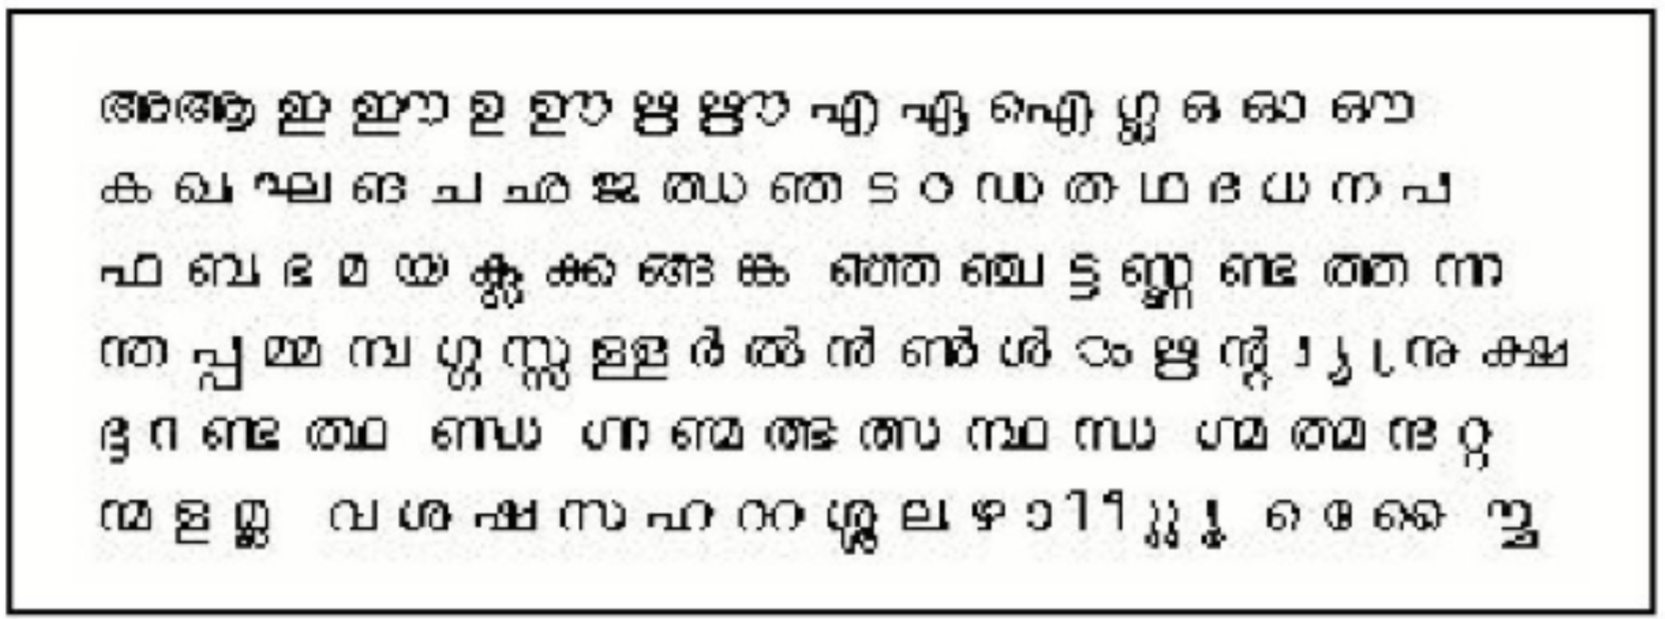
\includegraphics[width=12cm , height= 5cm]{dataset.png}    
		\caption{Malaylam characters}
		\label{fig1}
	\end{center}
\end{figure}
\vspace*{0.2cm}


Another dataset that we are using in this project is the images of the bus boards , The images of bus boards are captured and they are cropped in order to get the text content of that image alone. These are the images that are further enhanced to remove noise and make the image much more clear in order to provide it to an OCR system which is the proposed CNN model.


\paragraph{}
Data augmentation is done on these images in order to get Various images based on position, orientation and size. Data augmentation is a strategy that enables practitioners to significantly increase the diversity of data available for training models, without actually collecting new data. Image data augmentation that can be used to artificially expand the size of a training dataset by creating modified versions of images in the datasets. The Kera’s deep learning neural network library provides the capability to fit models using image data augmentation.

\section{System Architecture}
A system architecture or systems architecture is the conceptual model that defines the structure, behavior, and more views of a system. It is integral to understand the system architecture of a system in order to identify sub modules of the problem at hand and moreover the relationship between these components.

\paragraph{}
A block diagram is a diagram of a system in which the principal parts or functions are represented by blocks connected by lines that show the relationships of the blocks. They are heavily used in engineering in hardware design, electronicdesign, software design, and process flow diagrams. Block diagrams are typically used for higher level, less detailed descriptions that are intended to clarify overall concepts without concern for the details of implementation. They are typically used for higher level,less detailed descriptions that are intended to clarify overall concepts without concern for the details of implementation. Block diagrams rely on the principle of the black box where the contents are hidden from view either to avoid being distracted by the details or because the details are not known. We know what goes in, we know what goes out, but we can’t see how the box does its work. Thus block diagram can be used to represent the real time anomaly detection system.

\vspace*{0.1cm}
\begin{figure}[!h]
	\begin{center}
		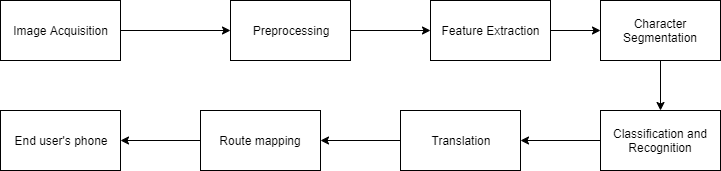
\includegraphics[width=12cm , height= 5cm]{overall.png}    
		\caption{System Architecture}
		\label{fig1}
	\end{center}
\end{figure}
\vspace*{0.2cm}

The diagram in Fig 4.1 has three broad divisions which are the image acquisition, feature extraction and recognition and classification. The images of bus boards are collected and are preprocessed to get better quality images. The basic features of these images are extracted are then transferred to the Deep Learning framework where recognition and classification of the Malayalam characters take place. The next stage is translation of these characters to English text. A route map is created consisting of all the bus stop destinations and is made available to the user. Once the destinations are obtained, the user is provided with the bus stops through which that particular bus travels. 

\section{UML Use case diagram}
Our principle use case of this project is to check whether the specific bus reaches the destination and provide a list of bus stops that the bus travels. This checking and listing of bus stops is done in our model.  The user provides the image of the bus, specifically bus board as input. The captured image is cropped in order to obtain the textual content from the image. Once the desired image format is obtained, our model detects the Malayalam script and translates them into English and provides the translated scripts to the user. The user is also provided with the bus stops that the specific bus travels. And also, the confirmation message whether the bus pass through the required bus stop requested by user.

\vspace*{0.1cm}
\begin{figure}[!h]
	\begin{center}
		\includegraphics[width=12cm , height= 5cm]{usecase6.png}    
		\caption{Use case diagram}
		\label{fig1}
	\end{center}
\end{figure}
\vspace*{0.2cm}

\section{OCR using Deep Learning Framework}
OCR is used to identify the character from human written text. To recognize the text segmentation of character is important stage. So here, we addressed different techniques to recognize the character. Segmentation problem of each language were different also handwritten character was also varied user to user, so it is necessary to make OCR systems more effective and accurate for segmentation. Comparative study concludes that deep learning technique gives good segmentation and gives better result in case with large dataset compares to other techniques.

In recognition system involves major five steps especially, Data collection, preprocessing, segmentation, features extraction and classification.
\begin{itemize}
\item Data Collection: For data acquisition many researchers used standard data sets available globally and some of researches uses own data sets for processing.
\item Pre - processing: In pre-processing phase many mathematical and morphological operations are applied on input document image for gay scale conversion, normalization, finalization, baseline detection, skew correction, slant detection, slant correction, noise removal and etc.
\item Segmentation: If the input document image consists of a sentence than that will be segmented into words than each word is consider as distinct substance.
\item Feature Extraction: The word is taken for further process, features like density features, structure based features, hierarchical features and other features are extracted from the input image. Which are the features extracted those are comparing with the training image features if the matching class is presented than that image is recognized.
\item Classification: for classification process classifiers are used like support Vector Machine (SVM), Convolutional Neural Network (CNN), Recurrent Neural Network (RNN) , Neural Networks, K Nearest Neighbour (KNN), Hidden Markov Model (HMM) and etc.
\end{itemize}


Deep learning is a powerful feature extraction method applied to extract the feature of the handwritten characters. Deep learning provides the task specific method, which inherits features from machine learning methods based on learning data representation. Learning can be supervised, semi supervised or unsupervised. It architectures such as Deep Neural Network, deep belief networks and RNN have been applied to fields natural language processing, computer vision, speech recognition, drug design, social network filtering, machine translation, bioinformatics, audio recognition, and where they have produced results comparable to and in some cases superior to human experts. There are many nonlinear hidden layers in deep neural networks, so the number of connections and parameters are very large. Apart from this, the train is also getting very difficult, too CNN is a class of deep neural network with relatively small parameters set and easy to train. The ability to model CNN correctly, the input data can be replaced with the number of layered layers and trainable parameters at each level and they also make the correct assumptions on the nature of the images. A CNN is a class of deep, feed-forward artificial neural networks that has successfully been applied to analysing visual imagery.

\section{Requirement Analysis}
The project contains several components to implement the proposed model. Several parameters were considered for the selection of the right tools for each of these components as follows:

\begin{itemize}
\item Image Acquisition: This will be done using a standard HD camera via a mobile phone.
\item Image processing: Numpy will be used for processing huge amounts of data due to it’s huge collection of high-level mathematical functions.
\item Feature Extraction: In order to extract only the features which are essential, feature detection algorithm is used. The project plans to use HOG algorithm for feature extraction.
\item Deep Learning Model: The project not only implements deployment of the deep learning model, but also training of the architecture. And since the model is on the computationally expensive side, it is very important that a very fast library is used for the project. Because of this reason and the reason, the project plans to use Keras as the Deep Learning library. 
\item Web Application: The project’s user platform will be a web application. The project plans to use Android studio for creating android applications seamlessly.
\end{itemize} 


\newpage
\renewcommand\chaptername{CHAPTER}
\chapter{METHODOLOGY}
The project undertaken contains an array of sub tasks and a limited 
time to carry out in order to finish the project on time with the 
mentioned specifications. So that, managing the various tasks by 
scheduling and allotting to the right person is very crucial. With 
various components like the image acquistion, dataset creation, feature 
extraction and the deep learning framework and deployment into a web 
application, a modern project management methodology was required for 
our successful completion.

\paragraph{}
With the rising popularity of agile development methodology, and since our projects had lesser iterations to be done, we decided to adopt the Agile-Kanban methodology for managing our project. The management of the project was done on the open source platform, Ora Project Management. The basic Agile-Kanban methodology consists of four phases of a process, i.e To-Do, In-Progress, Testing, and Backlog. The tasks that are tested and validated are moved to the Done section. In this methodology of project management, each process moves in like they are moving through the assembly line and it is a methodology that has been proved to be very effective in not only the software industry, but others as well. Using the tool helps us specify various things about the tasks like, a detailed description about the task, checklist of things to ensure the task completion, type of task, deadline, the person it is assigned to, etc. Overall it is a very powerful free tool that has eased project tracking and management for us. We have adopted the idea of daily stand-ups to keep track of each of our progress. This has helped us a lot to keep the project work flow along with other academic tasks. Also, this is very effective in figuring out problems and hurdles in our tasks. We also record the minutes of our short stand-up sessions. We are also planning to deploy it on a docker container, and try out some updates to our product and hence adapt some of the Dev-Ops principles.

\newpage
\renewcommand\chaptername{CHAPTER}
\chapter{CONCLUSION}
Rapid economic development exerts pressure on all infrastructure services , especially the bus services, which is vital for economic efficiency and social sustainability, particularly transport infrastructure. Public Bus transport in India  play a crucial role in significant role in social cohesion, helping people, especially those on low incomes, access education, work and health-care. Despite being such a widely used mode of transport, it is unfortunate for the foreigners to not be able to take complete advantage of such a great service. The foreigners, in addition to the people who are unable to comprehend the native language, will be having a hard time trying to understand the different locations the bus will be travelling to. Hence, the resultant application to be developed by this project is mainly intended for this particular group of people. With the concept of image enhancement, CNN and language translation, the users will be able to get a complete understanding regarding the schedule of the bus, just by providing the image of the bus board as input. This solution is to be implemented as an android application. Since almost every individual in today’s world has a cellphone in possession and also with the software being developed as an android application, it can be downloaded and used by anyone, anywhere, on any bus. This free of cost, easily available, extremely easy to use application can grab the attention of people from all around the country, thereby making it a popular and feasible solution. 

\paragraph{}
The project aims at training the model from scratch apart from using standard weights. There are other tasks like testing the database and the analytics platform. Each of the team member is assigned tasks on different areas of the project and the coordination for completing the tasks till now was very good. This flow is expected to continue till the end of the project. The team will be actively reviewing for possible issues and the time-line allows enough time for possible issues to be fixed.

\newpage
\addcontentsline{toc}{chapter}{REFERENCES}
\renewcommand\bibname{\textbf{REFERENCES}}
\bibliographystyle{ieeetr}

\begin{thebibliography}{2}
\bibitem{Jader} 
Jaderberg M, Simonyan K, Vedaldi A et al (2016) Reading text in the wild with convolutional neural networks. Int J Comput Vis 116(1):1-20 MathSciNetCrossRefGoogle Scholar

\bibitem{Goodfellow}
Goodfellow I J, Bulatov Y, Ibarz J, et al (2013) Multi-digit number recognition from street view imagery using deep convolutional neural networks. arXiv preprint arXiv:1312.6082Google Scholar

\bibitem{Hu}
Hu B, Lu Z, Li H, et al (2014) Convolutional neural network architectures for matching natural language sentences. Advances in Neural Information Processing Systems. 2042-2050Google Scholar


\bibitem{Nas}
Nasrabadi NM (2007) Pattern recognition and machine learning. Journal of Electronic Imaging 16(4):049901MathSciNetCrossRefGoogle Scholar

\bibitem{Cire}
Ciresan DC, Meier U, Masci J et al (2011) Flexible, high performance convolutional neural networks for image classification. IJCAI Proceedings-International Joint Conference on Artificial Intelligence 22(1):1237Google Scholar


\bibitem{Le}
LeCun Y, Bottou L, Bengio Y et al (1998) Gradient-based learning applied to document recognition. Proc IEEE 86(11):2278–2324CrossRefGoogle Scholar

\bibitem{He}
He K, Zhang X, Ren S, et al (2016) Identity Mappings in Deep Residual Networks. Computer Vision – ECCV 2016. Springer International Publishing, pp. 630–645Google Scholar

\bibitem{Xie}
Xie S, Girshick R, Dollar P, et al (2016) Aggregated Residual Transformations for Deep Neural Networks. 5987-5995Google Scholar

\bibitem{Jane}
Lane N D, Bhattacharya S, Georgiev P et al (2015) An Early Resource Characterization of Deep Learning on Wearables, Smartphones and Internet-of-Things Devices. International Workshop on Internet of Things Towards Applications. ACM, 7-12Google Scholar

\bibitem{Jenis}
Jenis J. Macwan, Mukesh M. Goswami, Archana N. Vyas, “A Survey on Offline Handwritten North Indian Script Symbol Recognition”, International Conference on Electrical, Electronics, and Optimization Techniques (ICEEOT) - 2016. 

\bibitem{Shruthi}
Shruthi A , M S Patel,” Offline Handwritten Word Recognition using Multiple Features with SVM Classifier for Holistic Approach” , International Journal of Innovative Research in Computer and Communication Engineering, June 2015.

\bibitem{Akm}
Akm Ashiquzzaman and Abdul Kawsar Tushar,” Handwritten Arabic Numeral Recognition using Deep Learning Neural Networks”, 2011.

\bibitem{Dar}
Darmatasia and Mohamad Ivan Fanany," Handwriting Recognition on Form Document Using Convolutional Neural Network and Support OPTICAL CHARACTER - P. Bhatt and I. Patel 65 Vector Machines", 2017 Fifth International Conference on Information and Communication Technology (ICoICT), 2017.


\bibitem{Cha}
Chaouki Boufenar , Adlen Kerboua, Mohamed Batouche,"Investigation on deep learning for off-line handwritten Arabic character recognition", Cognitive Systems Research, 2017.

\bibitem{Wei}
WeixinYang , LianwenJin , DachengTao , ZechengXie , ZiyongFeng, "A new training method to enhance deep convolutional neural networks for large-scale unconstrained handwritten Chinese character recognition”". 

\bibitem{Jan}
Jangid, Mahesh, et al. "SVM classifier for recognition of handwritten Devanagari numeral.” Image Information Processing (ICIIP), 2011 International Conference on. IEEE, 2011. 

\bibitem{Bha}
Bhattacharya, U., et al., "Neural combination of ANN and HMM for Handwritten Devanagari numeral recognition." Tenth International Workshop on Frontiers in Handwriting Recognition. Suvisoft, 2006. 

\bibitem{Meh}
Mehrotra, Kapil, et al., "Unconstrained handwritten Devanagari character recognition using convolutional neural networks." Proceedings of the 4th International Workshop on Multilingual OCR. ACM, 2013. 



\end{thebibliography}


\end{document}